This section describes how changes in the environment are defined, and how they are used to calculate the ESI.
\subsection{Changes}
The difference that is measured is defined as a \textit{change in how the robot perceives its environment}. The change is measured against the map the robot has of said environment. 
This is an important definition, with three major aspects. The first is that there can be a lot of changes to an environment, but if the robot does not sense it, then the changes 
by definition have no impact on the robot's ability to localize itself. 
The second is that it makes the index agnostic to which localization method is used, and which sensor modalities are available. A difference in observed visual features (I.e. SIFT) 
can be used just as well as geometric lidar, radar or sonar points, both 2D and 3D. The third is that changes that *could* be sensed but aren't, should not affect the index. 
Changes that happen outside the sensor coverage can naturally not be detected, and so they have no effect on localization. Unseen changes may also change back to the initial state 
before they are even noticed. The metric should as mentioned apply to any kind of sensors used, but since MiR robots localize via 2D Lidar, this will be the sensor modality used 
from here on. The reference map could likewise be of any kind (graph based, geometry based, grid based, etc), but for this project, the (occupancy) grid-based map is selected. 

Any physical object can result in a change in the environment by being either removed, added, moved, deformed or alter how it interacts with the sensor. 
However, this can be simplified to just Removed and Added. Any of the last three changes (moved, deformed, different sensor interaction) can be considered as a combination 
of removing the original item, and adding in the new. The distinction makes no difference from the robots point of view. Finally, an object can be observed to be 
exactly as expected - this will be denoted as Matched. There are many ways a sensor reading can be categorized as either of these, and the method chosen is by no means 
the only viable option. 

\subsection{The Environment Similarity Index (ESI)}
The index is a ratio, based on the current pose estimate from the robots localization module - for this paper, AMCL. On every laser-scan callback, each ray point is evaluated: 
Is it close to an expected obstacle in the map? If yes, count as a \underline{Matched}; else, count as an \underline{Added}. This tells us that an object has been added to the environment 
that is not on the map.  In addition, all laser rays that returned a value are traced in the map from the scanner and outwards to detect obstacles that they \textit{should} 
have hit but didn't. These objects count towards \underline{Removed} to indicate that something on the map has been removed from the environment. 
These classifcations are then used to calculate the ESI score; Figure X provides an overview of the classification.

\begin{figure}[htbp]
    \centerline{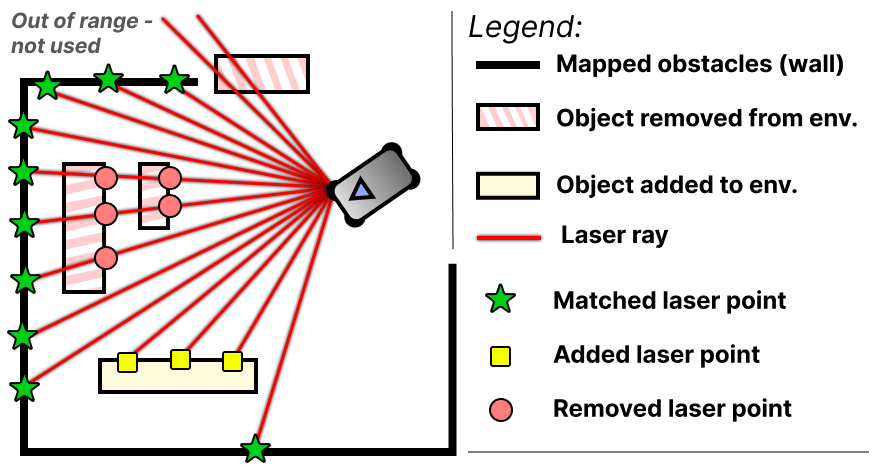
\includegraphics[width=\columnwidth]{figures/figure_1_esi_example.png}}
    \caption{Example of a figure caption.}
    \label{fig1}
\end{figure}

\subsection{Formal Definition}
\textbf{Matched:}
Let $S$ be a 1D vector representing a single scan containing $n_s = |S|$ geometric scan points $s: S = (s_0, s_1, \dots, s_{n_s-1})$.
Only scan points that return a value within min and max range are considered valid. The points are indexed by $i$ where $0 \le i < n_s$.
Let $G$ be a 1D vector representing the discrete geometric reference map, flattened from its original $N$-dimensional form:

$G = (g_0, g_1, \dots, g_{n_g-1})$
The occupancy value at index $i$ is $v(g_i)$, which equals 1 if $g_i$ represents an obstacle, and 0 otherwise.
The assignment $\lambda(i)$ returns the index in $G$ with the shortest distance to the scan point $s_i$:
\begin{equation}
\lambda(i)=\underset{0\le j<n_g}{\text{arg min }}d(s_i,g_j)
\end{equation}
The distance $d(p_1, p_2)$ is the Euclidean distance between two points in $R^N$, where $N$ depends on the map representation, but any distance metric can be used.
Let $T$ be a variable distance threshold. It is based on the expected yaw noise $\gamma$ [rad] and the range of the scan point $r(s_i)$:
\begin{equation}
T(i)=\sin(\gamma)*r(s_i)
\end{equation}
Define a match as:
\begin{equation}
\chi_M(i) = \begin{cases} 1 & \text{if } d(s_i, g_{\lambda(i)}) < T(i), \\ 0 & \text{otherwise}. \end{cases}
\end{equation}
The number of matches for a single scan is then:
\begin{equation}
M = \sum_{i=0}^{n_s-1} \chi_M(i)
\end{equation}

\textbf{Added:}
All valid scan points are classified as either Match or Added. Therefore, the number of added is simply the number of valid scan points minus the number of matches:
\begin{equation}
A = n_s - M
\end{equation}

\textbf{Removed:}
Each valid scan point defines the endpoint of a line from the scanner to that point, as seen in the world frame.
The laser ray $L$ contains all the discrete map points in $G$ that lie on that line:
$L = (l_0, l_1, \dots, l_{n_r-1})$ where $l_0$ is closest to the scanner.
We define a removed point to be every rising edge (going from free to occupied) that the ray encounters from the scanner and out.
Define removed as:
\begin{equation}
\chi_R(j) = \begin{cases} 1 & \text{if } v(l_j) = 1 \text{ and } v(l_{j-1}) = 0 \\ 0 & \text{otherwise}. \end{cases}
\end{equation}
The count of removed items (first encounters) in a scan with $k$ rays is then:
\begin{equation}
R = \sum_{k}\sum_{j=1}^{n_r^{(k)}-1} \chi_R^{(k)}(j)
\end{equation}

\textbf{ESI:}
The ESI score for a single scan S is then defined as:
\begin{equation}
ESI \in [0,1] = \frac{M}{M+A+R}
\end{equation}
and since $n_s = M + A$, the final expression becomes:
\begin{equation}
ESI = \frac{\sum_{i=0}^{n_s-1}\chi_M(i)}{n_s+\sum_{k}\sum_{j=1}^{n_r^{(k)}-1} \chi_R^{(k)}(j)}
\end{equation}

If the scan only sees matches, the ratio is 1/1 = 1, indicating a perfect match with the map.
Both added and removed points increases the denominator equally, driving the index down.  
Note how this reflects reality; there is no upper limit to how much you can change an environment; you can always use a sensor 
with a greater range and higher resolution and then add more items that are not mapped. 
The index therefore converges towards zero as more changes are made, but it will only be exactly zero if it sees zero matches.
The index can be calculated for any number of measurements per sensor update, and can be used for any given localization module. 

